
%(BEGIN_QUESTION)
% Copyright 2010, Tony R. Kuphaldt, released under the Creative Commons Attribution License (v 1.0)
% This means you may do almost anything with this work of mine, so long as you give me proper credit

Suppose we have an Allen-Bradley model ``SLC 500'' PLC connected to a three switches and two AC loads (a lamp and a solenoid coil) as shown in this illustration:
Her ser du en Allen-Bradley model ``SLC 500'' PLS koblet til tre innganger og to utganger. Inngangene består av to sensorer og en trykknapp. Utgangene består av en solenoid og et lys. 

$$\includegraphics[width=15.5cm]{i04527x01.eps}$$

The following is the PLC's program as it appears printed on paper.  From this information, determine the status of the lamp and of the solenoid coil provided a process pressure of 9 bar, a process temperature of 186 $^{o}$C, and an unpressed pushbutton switch:

$$\includegraphics[width=5.5cm]{i04527x02.eps}$$

\underbar{file i04527}
%(END_QUESTION)





%(BEGIN_ANSWER)

Both the lamp and the solenoid coil will be energized:

$$\includegraphics[width=15.5cm]{i04527x03.eps}$$

%(END_ANSWER)





%(BEGIN_NOTES)









\vskip 20pt \vbox{\hrule \hbox{\strut \vrule{} {\bf Virtual Troubleshooting} \vrule} \hrule}

This question is a good candidate for a ``Virtual Troubleshooting'' exercise.  Presenting the diagram to students, you first imagine in your own mind a particular fault in the system.  Then, you present one or more symptoms of that fault (something noticeable by an operator or other user of the system).  Students then propose various diagnostic tests to perform on this system to identify the nature and location of the fault, as though they were technicians trying to troubleshoot the problem.  Your job is to tell them what the result(s) would be for each of the proposed diagnostic tests, documenting those results where all the students can see.

During and after the exercise, it is good to ask students follow-up questions such as:

\begin{itemize}
\item{} What does the result of the last diagnostic test tell you about the fault?
\item{} Suppose the results of the last diagnostic test were different.  What then would that result tell you about the fault?
\item{} Is the last diagnostic test the best one we could do?
\item{} What would be the ideal order of tests, to diagnose the problem in as few steps as possible?
\end{itemize}


\vfil \eject

\noindent
{\bf Prep Quiz:}

$$\includegraphics[width=15.5cm]{i04527x01.eps}$$

The following is the PLC's program as it appears printed on paper.  From this information, determine the status of the lamp and of the solenoid coil provided a process pressure of 130 PSI, a process temperature of 186 $^{o}$F, and someone continuously pressing the pushbutton switch:

$$\includegraphics[width=15.5cm]{i04527x02.eps}$$


%INDEX% PLC, relating I/O status to virtual elements

%(END_NOTES)


